
\documentclass{article}

\usepackage[french]{babel}
\usepackage[utf8]{inputenc}
\usepackage{graphicx}
\usepackage{amssymb} % for R
%%%%%%%%%%%%%%%% Lengths %%%%%%%%%%%%%%%%
\setlength{\textwidth}{15.5cm}
\setlength{\evensidemargin}{0.5cm}
\setlength{\oddsidemargin}{0.5cm}

%%%%%%%%%%%%%%%% Variables %%%%%%%%%%%%%%%%
\def\projet{1}
\def\titre{Méthodes de calcul numérique }
\def\groupe{4}
\def\equipe{2}
\def\responsible{Kamgang Nintcheu David}
\def\secretary{Langlais Hugo}
\def\others{Roger Gaetan, Medina Enzo}
\def\cordicPythonFile{cordic.py}


\begin{document}

%\maketitle

%%%%%%%%%%%%%%%% Header %%%%%%%%%%%%%%%%
\noindent\begin{minipage}{0.98\textwidth}
  \vskip 0mm
  \noindent
  { \begin{tabular}{p{7.5cm}}
      {\bfseries \sffamily
        Projet \projet} \\ 
      {\itshape \titre}
    \end{tabular}}
  \hfill 
  \fbox{\begin{tabular}{l}
      {~\hfill \bfseries \sffamily Groupe \groupe\ - Equipe \equipe
        \hfill~} \\[2mm] 
      Responsable : \responsible \\
      Secrétaire : \secretary \\
      Codeurs : \others
    \end{tabular}}
  \vskip 4mm ~

  ~~~\parbox{0.95\textwidth}{\small \textit{Résumé: } \sffamily 
  Ce projet consiste à étudier les calculs numériques sur machine. 
  La première partie se focalise sur l'erreur relative engendré par les calculs machines. 
  La seconde en revanche, étudie les algorithmes par des machines possédant des ressources limités (mémoire, puissance de calcul).
}
  \vskip 1mm ~
\end{minipage}

%%%%%%%%%%%%%%%% Main part %%%%%%%%%%%%%%%%

\section*{Partie I - Représentation des nombres en machine}

\subsection*{Représentation décimale réduite}
Dans un premier temps, on crée la fonction rp(x, p) qui nous permet de récupérer la représentation décimale réduite d'un nombre en fonction d'une précision donnée.

Pour cela, nous récupérons d'abord la notation scientifique du nombre x. Puis nous sélectionnons seulement les p premières décimales de ce nombre et enfin nous multiplions le résultat obtenu par la puissance de dix perméttant un résultat du même ordre de grandeur que le x passé en paramètre.

\subsection*{Opérations usuelles en représentation décimale réduite}

Pour simuler les opérations usuelles (addition ou multiplication) en représentation décimale réduite, on crée une fonction qui prends en argument les deux nombres et la précision demandé (On part du principe que la précision est commune aux deux nombres).

On commence par récupérer la représentation décimale réduite des deux nombres via la fonction précédente. Ensuite, on calcule la somme (resp. multiplication) et on en calcule la représentation décimale réduite. On est obligé de réutiliser la fonction car la somme (resp.multiplication) de deux nombres ne donne pas nécessairement un nombre avec la bonne précision. \\

Exemple :
Une précision de 3 sur les nombres 8.547 et 3.589 nous donne 8.54 et 3.59. En les sommant, on obtiens 12.13 qui à une précision de 4. On est donc bien obligé d'appeler une seconde fois la fonction rp() pour une obtenir une précision de 3.

\subsection*{Erreur relative}

On calcule l'erreur relative de la somme et de la multiplication donné par les formules :
\\

Erreur relative sur la somme:
\begin{equation}
\delta_{s}(x,y) = \frac{ \left |  (x+y)_{reel}\ - \ (x+y)_{machine} \right | }{\left |  (x+y)_{reel} \right | }
\label{erreur_relative_sur_la_somme}
\end{equation}

Erreur relative sur le produit:
\begin{equation}
\delta_{p}(x,y) = \frac{ \left |  (x*y)_{reel}\ - \ (x*y)_{machine} \right | }{\left |  (x*y)_{reel} \right | }
\label{erreur_relative_sur_le_produi}
\end{equation}

Ici, on considère le résultat "réel" comme étant celui calculé par python. Le résultat machine correspond à notre calcul précédent. On arrive alors à obtenir une erreur relative qui nous permet d'examiner la précision de notre calcul. 
Sans surprise, plus la précision est forte, plus l'erreur relative est faible.

\subsection*{Graphes d'erreur relative}

On pose une précision égale à 3 pour n'avoir ni une précision trop forte (impliquant une erreur relative trop faible) ni une précision trop faible (impliquant une erreur relative trop forte).

Les figures \ref{fig:erreur_sur_la_somme_2} et \ref{fig:erreur_sur_le_produit_2} ci-dessous représentent les erreurs relatives ${x = 1}$, soit une précision supérieure aux décimales du nombre, et ${x = 5.7555}$ soit une précision inférieure aux décimales du nombre. On remarque que l'erreur est maximal quand la somme à calculer est nulle. De plus cette erreur est bien plus grande dans le cas où ${x=5.7555}$ que dans le cas où ${x=1}$ cela peut s'expliquer par le fait que dans ce deuxième cas x possède plus de décimales que la précision choisi ainsi le nombre étant tronqué l'erreur relative en sera donc augmentée. 

\begin{figure}[ht]
    \begin{minipage}{0.48\textwidth}
        \centering
        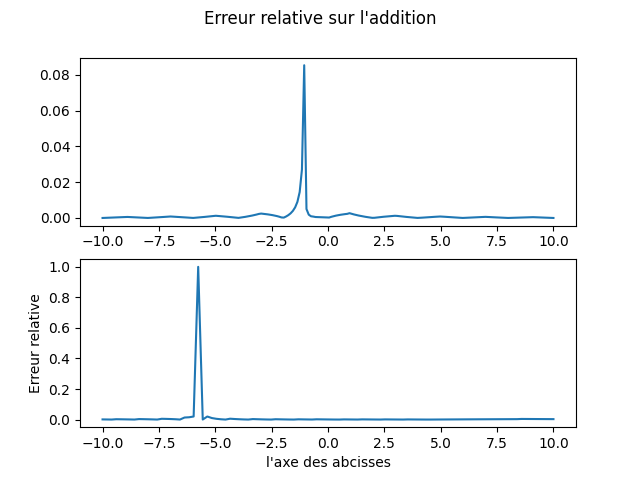
\includegraphics[scale=0.48]{images/erreur_add.png}
        \caption{Erreur relative sur la somme}
        \label{fig:erreur_sur_la_somme_2}
    \end{minipage}\hfill
    \begin{minipage}{0.48\textwidth}
        \centering
        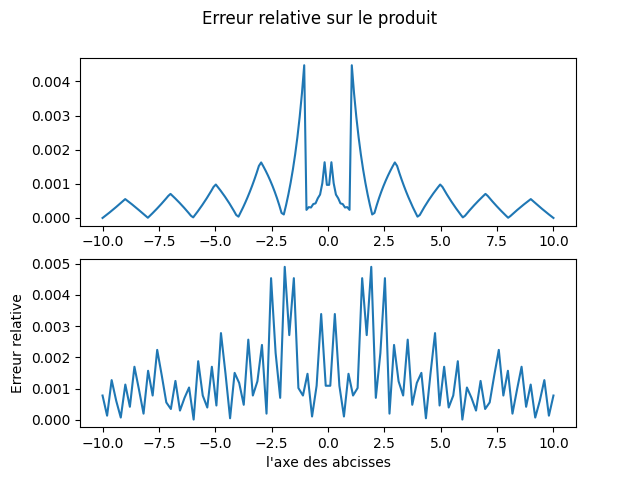
\includegraphics[scale=0.48]{images/erreur_prod.png}
        \caption{Erreur relative sur le produit}
        \label{fig:erreur_sur_le_produit_2}
    \end{minipage}
\end{figure}

Nous avons conservé les mêmes valeurs de x pour l'erreur relative sur le produit. On peut remarquer que les résultats sont bien moins prévisibles et que surtout l'erreur relative atteinte est beaucoup plus faible. 

\subsection*{Logarithme}

On commence par simplifier $log(2)$ avec l'équation \ref{eq:reduction_log} afin d'éviter les soustractions et donc pour limiter les erreurs : 

\begin{equation}
\frac{1}{n}-\frac{1}{n+1}=\frac{1}{n(n+1)} \rightarrow log(2) = \sum_{k=1}^{\infty}\frac{1}{2k(2k-1)}
\label{eq:reduction_log}
\end{equation}

En utilisant le critère spécial des séries alternées, on peut majorer l'erreur absolue $\epsilon$ de la somme des $N$ premiers termes de la série. Obtient donc l'équation \ref{eq:CSSA_majoration} :

\begin{equation}
    \epsilon \leq \frac{1}{2N+1}
    \label{eq:CSSA_majoration}
\end{equation}

Par conséquant, pour obtenir une précision sur p décimales, on a besoin d'aller à un N égal à ${10^{p}}$. 

Dès lors que l'on arrive à calculer un logarithme approché (en fonction de la précision), on peut en déduire l'erreur relative en fonction de la précision. On affiche sur un graphe l'erreur relative jusqu'à la précision 6 (On ne voit plus de différence avec une précision 7 ou au dessus, l'erreur relative étant inférieur à ${1.10^{-6}}$. Nous obtenons donc les figures suivantes \ref{fig:log_prec} et \ref{fig:compare_log}.

\begin{figure}[ht]
    \begin{minipage}{0.48\textwidth}
        \centering
        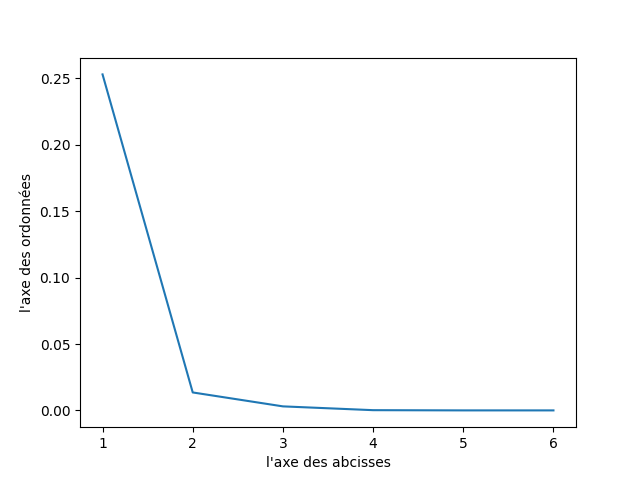
\includegraphics[scale=0.5]{images/erreur_relative.png}
        \caption{Erreur relative du log en fonction de la précision}
        \label{fig:log_prec}
    \end{minipage}\hfill
    \begin{minipage}{0.48\textwidth}
        \centering
        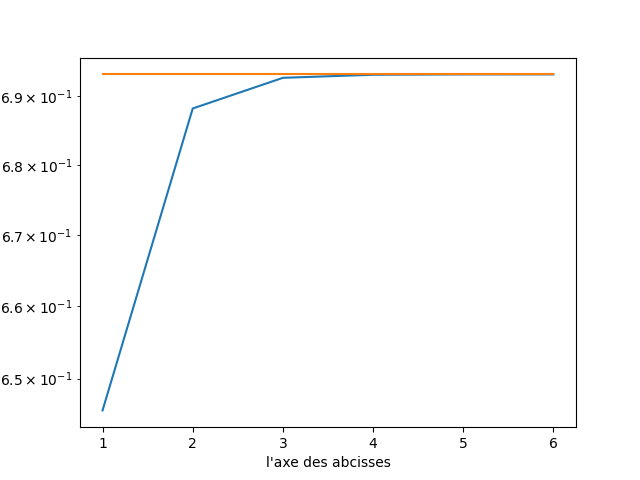
\includegraphics[scale=0.5]{images/graphes_log.png}
        \caption{Les deux log calculés, valeur réelle et valeur approchée en fonction de la précision}
        \label{fig:compare_log}
    \end{minipage}
\end{figure}


\section*{Partie II - Algorithmes CORDIC}

Nous allons maintenant étudier les algorithmes de calcul CORDIC utilisées par les calculatrices, machines avec peu de ressources. Ces derniers doivent rester précis malgré leur grande optimisation.

\subsection*{Représentation des nombres sur calculatrice}

Dans une calculatrice, les nombres sont représentés en Binaire Code Decimal (ou BCD), une écriture binaire plus proche de notre représentation usuelle. Voici son principe : Les nombres sont représentés par des nombres décimaux et chaque chiffre est codé sur 4 bits. \\

Voici un exemple d'écriture du nombre 12 : \\

\begin{tabular}{ c | c | c c }
    \label{exemple_de_representation_pour_12}
   Base 10 & Binaire &   \multicolumn{2}{c}{Binaire Code Decimal}\\ \hline
    12 & 1100 & $\underbrace{0001}$ & $\underbrace{0001}$ \\
    & & 1 en binaire & 2 en binaire \\
 \end{tabular} \\ \\ 

Cette représentation présente certains avantages et inconvénients par rapport à l'écriture binaire dite classique, ils sont les suivants : \\

Avantages :
\begin{itemize}
    \item La multiplication et la division par 10n est plus rapide : shift left ou droit de 4n bits (avec n entier).
    \item Toutes les fonctions 'standards' peuvent se ramener aux quatre fonctions suivantes :  ln, exp, tan, arctan
    \item Possibilité d'utiliser les algorithmes CORDIC qui permettent d'avoir une précision de plus de 12 chiffres avec seulement une quinzaine de valeurs précalculées.
\end{itemize}

\vspace{1em}

Inconvénients :
\begin{itemize}
    \item La multiplication et la division par 2n est plus lente : le shift de 1 bit ne multiplie ou divise plus par 2 (avec n entier)
    \item Un même nombre x, prends plus de place en mémoire : on a besoin de 4n bits contre $log2(x) +1$ (avec n le nombre de chiffres dans x en représentation décimale)
    \item L'algorithme CORDIC nécessite certaines valeurs précalculées, elles prennent donc un espace mémoire supplémentaire et il faut possiblement les calculer.
    \item La précision des calculs dépend de celle des valeurs précalculées.
\end{itemize}

\subsection*{Analyse des algorithmes CORDIC}

L'algorithme CORDIC est basé sur 2 concepts importants :
\begin{itemize}
    \item La recherche : On s'approche de la valeur cible en ajoutant des valeurs précalculées de plus en plus petites
    \item Le remplacement des multiplications coûteuses en temps par des shifts
\end{itemize}

\vspace{1em}

Technique générale :
\begin{itemize}
    \item Le nombre en entrée noté x peut se décomposer sous un produit partiel (pour ln et exp) ou une somme partiel (pour tan et arctan) des valeurs précalculés
    \item On se sert de ces produits ou sommes pour exploiter les developements  limités à l'ordre 1 des fonctions considérées. Ainsi on approche x en sommant les puissances de 10 (pour une représentation BCD), pondérés par un terme dépendant de la fonction
    \item Pour chaque terme sommé, on ajoute un terme précalculé au résultat, pondéré par un terme dépendant de la fonction
    \item On retourne le résultat en ajoutant un terme d'erreur
\end{itemize}

\vspace{1em}

Cette technique est efficace car les valeurs précalculés et l'approche du nombre utilisent des multiplications et des divisions par des puissances de 10. Grâce à l'écriture BCD, lors de l'exécutions de l'algorithlen, la calculatrice ne fait presque qu'exclusivement des shift très peu coûteux.

\subsection*{Implémentation des algorithmes sous Python}

Nous implémentons les algorithmes dans le fichier \cordicPythonFile. Nous utilisons les pseudos algorythmes données dans les ressources du sujet afin d'implémenter nos algorythmes. Les valeurs précalculées sont générés grâce au module numpy avec une précision de 17 chiffres significatifs, ce qui est supérieur au 12 chiffres de précision en sortie d'algorythme.

Nos algorithme sont divisé en deux parties. La première ramène la valeur en entrée dans l'interval où la méthode est applicable. Nous utilisons les décompositions données dans les ressources du sujet, en vérifiant préalablement que la décomposition sont bien équivalente. La seconde partie calcul et retourne le résultat en utilisant l'algorythme CORDIC.

La première partie est testé en comparant le résultat avec et sans réduction de l'interval (la seconde partie fonctionne en effet sur $\mathbb{R}$). Les résultats de la seconde partie sont comparés avec les valeur  obtenues avec WolfrAmalpha et l'implémentation des fonctions ln, exp, tan et arctan dans la librairie numpy de python. Les figures \ref{fig:figure_tan_moins_tan} et \ref{fig:compare_log} représentent une partie des résultats des tests :

\begin{figure}[!htb]
    \begin{minipage}{0.48\textwidth}
        \centering
        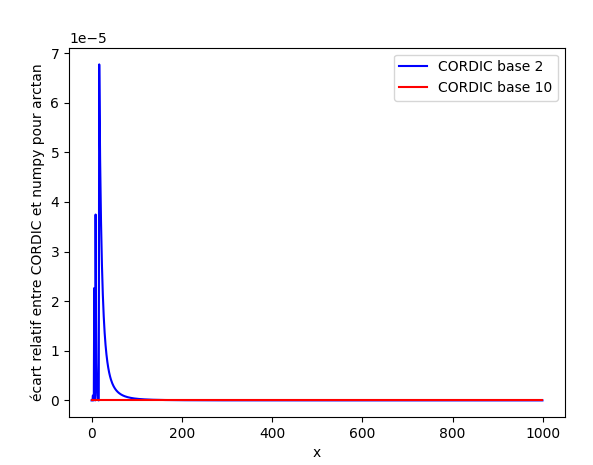
\includegraphics[scale=0.35]{images/ecart_atan.png}
        \caption{Différence entre l'implémentation CORDIC de arctan et celle du module numpy de python pour les bases 2 et 10}
        \label{fig:figure_tan_moins_tan}
    \end{minipage}\hfill
    \begin{minipage}{0.48\textwidth}
        \centering
        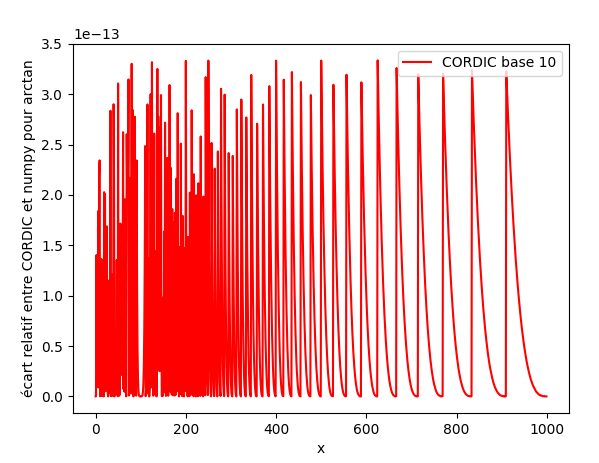
\includegraphics[scale=0.35]{images/ecart_arctan_base10.png}
        \caption{Différence entre l'implémentation CORDIC de arctan et celle du module numpy de python pour la bases 10 uniquement}
        \label{fig:figure_compare_log}
    \end{minipage}
\end{figure}

Nous remarquons que la précision des résulats dimminue change si nous utilisons la base 2, ce qui conduit à remplacer tous les $10^n$ par $2^n$. La figure \ref{fig:figure_tan_moins_tan} montre la différence de précision par rapport à numpy. Pour la base 10, l'écart maximal avec numpy est de l'ordre de $10^{-13}$, $10^{-5}$ pour la base 2. Les algorithmes ainsi modifiées se trouvent également dans le fichier \cordicPythonFile. De plus, avec un tableau plus grand, il est possible d'augmenter la précision du résultat (il faut également modifier les boucles while)

\subsection*{Problèmes lors de l’évaluation de fonctions usuelles en machine}

(P.167) Certaines fonctions usuelles, comme le sinus, ont un développement en série entière qui convergent lentement, ce qui rend le temps de calcul très long lors de l'évaluation informatique de la fonction à partir de sa série entière. Une façon de palier à ce problème est de faire une transformation d'Euler de cette série entière, ainsi on est sûr que les nouveaux termes de la séries obtenue convergent rapidement vers 0.\\
\begin{equation}
    \sum_{n=0}^\infty (-1)^n a_n = \sum_{n=0}^\infty (-1)^n \frac {\Delta^n a_0} {2^{n+1}}
    \label{eq:Euler_Transfo}
\end{equation}
ou
\begin{equation}
    \Delta a_n=a_{n+1}-a_n,\Delta^2 a_n=a_{n+2}-2a_{n+1}+a_n \dots
    \label{eq:Euler_Transfo_2}
\end{equation}

(P.186) Cependant en supposant  qu'on a réussi à avoir une implémentation efficace d'une fonction f, il reste à minimiser les erreurs liées à l'évaluation de ses dérivés. On a pour h proche de 0 : 
\begin{equation}
    f(x)\approx\frac{f(x+h)-f(x)}{h}
    \label{eq:derivée}
\end{equation}

Cette expression, provenant de la définition de la dérivée, est source d'erreurs informatiquement.

La première erreur est de choisir un h fixé et d’abandonner les termes restant du développement de Taylor de la fonction en x :
\begin{equation}
    \frac{f(x+h)-f(x)}{h}=f'+\frac{1}{2}hf''+ \dots
    \label{eq:developpement_de_Taylor}
\end{equation}

Pour palier à ce problème, il convient de choisir un h optimal de sorte a minimiser l'erreur dans notre expression approximative \ref{eq:derivée}. En notant $e_f$ la précision sur notre évaluation de $f$, le h optimal à choisir est pris $h = \sqrt{xe_f}$.
\newline

(P.186)La seconde erreur est due à l'encodage des nombre sur machine. Le h qu'on a choisi peut être arrondi. Pour des fonctions comme tan qui croît extrêmement vite au voisinage de $\frac{\pi}{2}$, ces arrondis peuvent donner des valeur de dérivés fausses. Une solution est de choisir alors h de sorte que $x+h$ dans \ref{eq:derivée} soit représentable en mémoire de manière exacte.


\end{document}
